\documentclass[12pt,a4paper]{article}
\usepackage[utf8]{vietnam}
\usepackage{amsmath,amssymb}
\usepackage{tabularx}
\usepackage{graphicx}
\usepackage{tikz}
\usetikzlibrary{calc,arrows.meta}
\usepackage{xcolor}
\usepackage{enumitem}
\usepackage{fancyhdr}
\usepackage[top=1.0cm, bottom=1.0cm, left=1.3cm, right=1.3cm]{geometry}
\usepackage[loigiai]{ex_test}
\SAOPTN{widthSA=2.6,heightSA=0.62}

\setlength{\headheight}{15pt}
\setlength{\parskip}{1pt}

\pagestyle{fancy}
\fancyhf{}
\rhead{\textit{Lời giải chi tiết -- Đề số 13}}
\lhead{\textit{Bộ đề ôn tập Giữa học kì I -- Toán 7}}
\cfoot{\thepage}

\begin{document}

\begin{center}
\textbf{\Large HƯỚNG DẪN CHẤM VÀ LỜI GIẢI CHI TIẾT}\\
\vspace{1mm}
\textbf{\large MÔN: TOÁN 7 -- ĐỀ SỐ 13}
\end{center}
\vspace{2mm}

\noindent\textbf{\large PHẦN I. CÂU TRẮC NGHIỆM NHIỀU PHƯƠNG ÁN LỰA CHỌN}

\vspace{1mm}
\begin{ex}
Kết quả của biểu thức $-\dfrac{3}{4} - \left(-\dfrac{1}{4}\right) - \dfrac{8}{7} - \dfrac{4}{7} - \dfrac{7}{7} + \dfrac{1}{3}$... sau khi thu gọn các phân số cùng mẫu là:
\choice
{$-\dfrac{37}{7}$}
{\True $-3$}
{$-\dfrac{25}{28}$}
{$-4$}
\loigiai{
Nhóm các số hạng có cùng mẫu số thích hợp ta được kết quả là $-3$.
}
\end{ex}

\begin{ex}
Kết quả của phép tính $\left(-\dfrac{2}{3}\right)^3$ là:
\choice
{$-\dfrac{6}{9}$}
{$\dfrac{8}{27}$}
{\True $-\dfrac{8}{27}$}
{$\dfrac{6}{9}$}
\loigiai{
Ta có $\left(-\dfrac{2}{3}\right)^3 = \dfrac{(-2)^3}{3^3} = -\dfrac{8}{27}$.
}
\end{ex}

\begin{ex}
Một hồ bơi có dạng hình hộp chữ nhật có các kích thước lần lượt là $15\text{ m}; 10\text{ m}; 1{,}8\text{ m}$. Thể tích hồ bơi là:
\choice
{\True $270\text{ m}^3$}
{$180\text{ m}^3$}
{$240\text{ m}^3$}
{$90\text{ m}^3$}
\loigiai{
Áp dụng công thức thể tích $V = a \cdot b \cdot c = 15 \cdot 10 \cdot 1{,}8 = 270\text{ m}^3$.
}
\end{ex}

\begin{ex}
Cho biểu thức $-\left(\dfrac{1}{12} - \dfrac{2}{5}\right)$, khi bỏ dấu ngoặc ta được:
\choice
{$\dfrac{1}{12} - \dfrac{2}{5}$}
{$-\dfrac{1}{12} - \dfrac{2}{5}$}
{$\dfrac{1}{12} + \dfrac{2}{5}$}
{\True $-\dfrac{1}{12} + \dfrac{2}{5}$}
\loigiai{
Bỏ dấu ngoặc có dấu trừ đằng trước: $-\left(\dfrac{1}{12} - \dfrac{2}{5}\right) = -\dfrac{1}{12} + \dfrac{2}{5}$.
}
\end{ex}

\begin{ex}
\immini{
Quan sát trục số sau, điểm $A$ biểu diễn số hữu tỉ nào?
\choice
{$1{,}3$}
{$4$}
{\True $\dfrac{4}{3}$}
{$\dfrac{4}{5}$}
}{
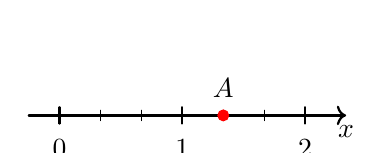
\begin{tikzpicture}[scale=1.3, line cap=round, line join=round]
    \draw[thick, ->] (-0.3,0) -- (2.8,0) node[below] {$x$};
    \foreach \x/\label in {0/0, 1.2/1, 2.4/2} {
        \draw[thick] (\x, 0.08) -- (\x, -0.08) node[below=2pt] {$\label$};
    }
    \foreach \x in {0.4, 0.8, 1.6, 2.0} {
        \draw (\x, 0.05) -- (\x, -0.05);
    }
    \filldraw[red] (1.6, 0) circle (1.5pt) node[above=3pt, black] {$A$};
\end{tikzpicture}
}
\loigiai{
Đoạn đơn vị từ $0$ đến $1$ được chia làm $3$ phần bằng nhau, mỗi phần là $\dfrac{1}{3}$. Điểm $A$ ở vạch thứ $4$, biểu diễn số $1 + \dfrac{1}{3} = \dfrac{4}{3}$.
}
\end{ex}

\begin{ex}
\immini{
Cho hình vẽ dưới đây, góc đối đỉnh với $\widehat{xOy}$ là góc nào?
\choice
{\True $\widehat{x'Oy'}$}
{$\widehat{xOy'}$}
{$\widehat{x'Oy}$}
{$\widehat{xOy}$}
}{
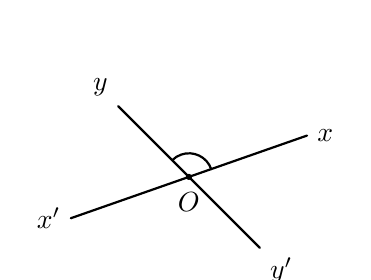
\begin{tikzpicture}[scale=0.75, line cap=round, line join=round]
    \coordinate (O) at (0,0);
    \draw[thick] (-2, -0.7) node[left] {$x'$} -- (2, 0.7) node[right] {$x$};
    \draw[thick] (-1.2, 1.2) node[above left] {$y$} -- (1.2, -1.2) node[below right] {$y'$};
    \filldraw[black] (O) circle (1.2pt) node[below=2pt] {$O$};
    \draw[thick] (O) ++(19.3:0.4) arc (19.3:135:0.4);
\end{tikzpicture}
}
\loigiai{
Hai đường thẳng $xx'$ và $yy'$ cắt nhau tại $O$. Tia đối của $Ox$ là $Ox'$, của $Oy$ là $Oy'$. Vậy góc đối đỉnh với $\widehat{xOy}$ là $\widehat{x'Oy'}$.
}
\end{ex}

\begin{ex}
Qua một điểm $M$ nằm ngoài đường thẳng $a$, kẻ được bao nhiêu đường thẳng song song với đường thẳng $a$?
\choice
{Có vô số đường thẳng}
{Không có đường thẳng nào}
{Có hai đường thẳng}
{\True Chỉ có một đường thẳng}
\loigiai{
Theo tiên đề Euclid, qua một điểm ở ngoài một đường thẳng chỉ có một đường thẳng song song với đường thẳng đó.
}
\end{ex}

\begin{ex}
Cho $\triangle ABC = \triangle DEF$. Biết $\widehat{A} = 33^\circ$. Khi đó:
\choice
{\True $\widehat{D} = 33^\circ$}
{$\widehat{B} = 33^\circ$}
{$\widehat{E} = 33^\circ$}
{$\widehat{F} = 33^\circ$}
\loigiai{
Vì $\triangle ABC = \triangle DEF$ nên các góc tương ứng bằng nhau, suy ra $\widehat{D} = \widehat{A} = 33^\circ$.
}
\end{ex}

\begin{ex}
Giá trị của $|-3|$ bằng:
\choice
{$-3$}
{\True $3$}
{$\dfrac{1}{3}$}
{$-\dfrac{1}{3}$}
\loigiai{
Giá trị tuyệt đối của số âm bằng số đối của nó: $|-3| = 3$.
}
\end{ex}

\begin{ex}
Làm tròn số $1{,}3781$ với độ chính xác $0{,}005$ được kết quả là:
\choice
{$1{,}37$}
{$1{,}4$}
{$1$}
{\True $1{,}38$}
\loigiai{
Độ chính xác $0{,}005$ yêu cầu làm tròn đến hàng phần trăm. Chữ số hàng phần trăm là $7$, chữ số liền sau là $8 \ge 5$ nên tăng $1$ đơn vị thành $1{,}38$.
}
\end{ex}

\begin{ex}
Số đỉnh của hình hộp chữ nhật là:
\choice
{$6$}
{\True $8$}
{$10$}
{$12$}
\loigiai{
Hình hộp chữ nhật gồm $4$ đỉnh ở mặt đáy trên và $4$ đỉnh ở mặt đáy dưới, tổng cộng có $8$ đỉnh.
}
\end{ex}

\begin{ex}
\immini{
Cho hình vẽ sau, biết $a \parallel b$ và $\widehat{A} = 45^\circ$. Số đo của góc $\widehat{B}_1$ bằng bao nhiêu?
\choice
{$145^\circ$}
{$45^\circ$}
{$35^\circ$}
{\True $135^\circ$}
}{
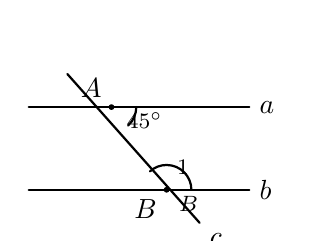
\begin{tikzpicture}[scale=0.7, line cap=round, line join=round]
    \draw[thick] (-1.5, 1.5) -- (2.5, 1.5) node[right] {$a$};
    \draw[thick] (-1.5, 0) -- (2.5, 0) node[right] {$b$};
    \draw[thick] (-0.8, 2.1) -- (1.6, -0.6) node[below right] {$c$};
    \filldraw[black] (0, 1.5) circle (1.2pt) node[above left] {$A$};
    \filldraw[black] (1.0, 0) circle (1.2pt) node[below left] {$B$};
    % Angle A
    \draw[thick] (0, 1.5) ++(0:0.45) arc (0:-48:0.45);
    \node[font=\footnotesize] at (0.6, 1.25) {$45^\circ$};
    % Angle B1
    \draw[thick] (1.0, 0) ++(0:0.45) arc (0:132:0.45);
    \node[font=\footnotesize] at (1.3, 0.4) {$1$};
    \node[font=\footnotesize] at (1.4, -0.25) {$B$};
\end{tikzpicture}
}
\loigiai{
Vì $a \parallel b$ nên góc $\widehat{A} = 45^\circ$ và góc $\widehat{B}_1$ ở vị trí trong cùng phía bù nhau: $\widehat{B}_1 = 180^\circ - 45^\circ = 135^\circ$.
}
\end{ex}


\setcounter{ex}{0}
\noindent\textbf{\large PHẦN II. CÂU TRẮC NGHIỆM ĐÚNG SAI}

\vspace{1mm}
\begin{ex}
Cho biểu thức $Q = \left(-\dfrac{1}{3}\right)^2 \cdot 9 + \left|-\dfrac{3}{5}\right| : \dfrac{3}{5} - \dfrac{1}{2}$. Xét tính đúng sai của các mệnh đề sau:
\choiceTF
{\True Giá trị của lũy thừa $\left(-\dfrac{1}{3}\right)^2$ bằng $\dfrac{1}{9}$}
{Giá trị tuyệt đối $\left|-\dfrac{3}{5}\right|$ bằng $-\dfrac{3}{5}$}
{\True Kết quả của phép tính $\dfrac{3}{5} : \dfrac{3}{5}$ bằng $1$}
{\True Giá trị của biểu thức $Q$ bằng $\dfrac{3}{2}$}
\loigiai{
\begin{itemize}[leftmargin=0.6cm, itemsep=1pt]
\item \textbf{a)} \textbf{Đúng}. Ta có $\left(-\dfrac{1}{3}\right)^2 = \dfrac{(-1)^2}{3^2} = \dfrac{1}{9}$.
\item \textbf{b)} \textbf{Sai}. Giá trị tuyệt đối luôn không âm, do đó $\left|-\dfrac{3}{5}\right| = \dfrac{3}{5}$.
\item \textbf{c)} \textbf{Đúng}. Thực hiện phép chia hai số bằng nhau: $\dfrac{3}{5} : \dfrac{3}{5} = 1$.
\item \textbf{d)} \textbf{Đúng}. Thay các giá trị vào: $Q = \dfrac{1}{9} \cdot 9 + 1 - \dfrac{1}{2} = 1 + 1 - \dfrac{1}{2} = \dfrac{3}{2}$.
\end{itemize}
}
\end{ex}

\begin{ex}
\immini{
Quan sát hình vẽ, biết $MN \perp yy'$ tại $M$ và $MN \perp zz'$ tại $N$; đường thẳng $xx'$ cắt $yy'$ tại $A$ và cắt $zz'$ tại $B$ sao cho góc $\widehat{xAy'} = 60^\circ$. Xét tính đúng sai của các mệnh đề sau:
\choiceTF
{\True Hai đường thẳng $yy'$ và $zz'$ song song với nhau}
{\True Số đo của góc $\widehat{yAB}$ bằng $60^\circ$}
{Số đo của góc $\widehat{ABz'}$ bằng $120^\circ$}
{\True Hai góc $\widehat{y'AB}$ và $\widehat{ABz}$ là hai góc so le trong và đều có số đo bằng $120^\circ$}
}{
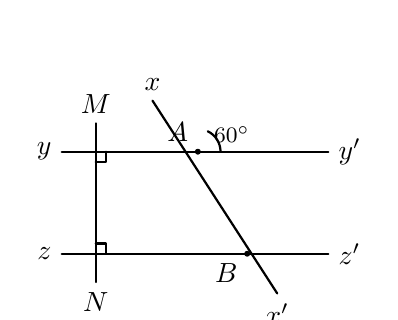
\begin{tikzpicture}[scale=0.72, line cap=round, line join=round]
    % Lines yy' and zz'
    \draw[thick] (-2.2, 1.8) node[left] {$y$} -- (2.5, 1.8) node[right] {$y'$};
    \draw[thick] (-2.2, 0) node[left] {$z$} -- (2.5, 0) node[right] {$z'$};
    % MN perpendicular
    \draw[thick] (-1.6, 2.3) node[above] {$M$} -- (-1.6, -0.5) node[below] {$N$};
    \draw[thick] (-1.6, 1.8) ++(0,-0.18) -- ++(0.18,0) -- ++(0,0.18);
    \draw[thick] (-1.6, 0) ++(0,0.18) -- ++(0.18,0) -- ++(0,-0.18);
    % Line xx'
    \draw[thick] (-0.6, 2.7) node[above] {$x$} -- (1.6, -0.7) node[below] {$x'$};
    \filldraw[black] (0.2, 1.8) circle (1.2pt) node[above left] {$A$};
    \filldraw[black] (1.07, 0) circle (1.2pt) node[below left] {$B$};
    % Angle xAy' = 60
    \draw[thick] (0.2, 1.8) ++(0:0.4) arc (0:64:0.4);
    \node[font=\footnotesize] at (0.8, 2.1) {$60^\circ$};
\end{tikzpicture}
}
\loigiai{
\begin{itemize}[leftmargin=0.6cm, itemsep=1pt]
\item \textbf{a)} \textbf{Đúng}. Vì $yy' \perp MN$ và $zz' \perp MN$ nên $yy' \parallel zz'$.
\item \textbf{b)} \textbf{Đúng}. Tại đỉnh $A$, hai góc $\widehat{yAB}$ và $\widehat{xAy'}$ là hai góc đối đỉnh nên $\widehat{yAB} = \widehat{xAy'} = 60^\circ$.
\item \textbf{c)} \textbf{Sai}. Vì $yy' \parallel zz'$ nên $\widehat{ABz'} = \widehat{xAy'} = 60^\circ$ (hai góc đồng vị), do đó khẳng định $120^\circ$ là sai.
\item \textbf{d)} \textbf{Đúng}. Vì $\widehat{y'AB} + \widehat{xAy'} = 180^\circ \implies \widehat{y'AB} = 120^\circ$. Do $yy' \parallel zz'$ nên hai góc so le trong $\widehat{y'AB} = \widehat{ABz} = 120^\circ$.
\end{itemize}
}
\end{ex}


\setcounter{ex}{0}
\noindent\textbf{\large PHẦN III. CÂU HỎI TRẢ LỜI NGẮN}

\vspace{1mm}
\begin{ex}
Cho $\widehat{xOy} = 70^\circ$, $Ot$ là tia phân giác của $\widehat{xOy}$. Số đo $\widehat{xOt}$ bằng bao nhiêu độ? \shortans{$35^\circ$}
\loigiai{
Vì $Ot$ là tia phân giác của $\widehat{xOy}$ nên $\widehat{xOt} = \dfrac{\widehat{xOy}}{2} = \dfrac{70^\circ}{2} = 35^\circ$.

\textbf{Đáp số:} $35^\circ$
}
\end{ex}

\begin{ex}
Tìm số hữu tỉ $x$, biết: $\left|2x - \dfrac{1}{3}\right| - \dfrac{1}{2} = \dfrac{1}{6}$. \shortans{$x = \dfrac{1}{2} \text{ hoặc } x = -\dfrac{1}{6}$}
\loigiai{
Ta có $\left|2x - \dfrac{1}{3}\right| = \dfrac{1}{6} + \dfrac{1}{2} = \dfrac{2}{3}$.\par $\bullet$ TH1: $2x - \dfrac{1}{3} = \dfrac{2}{3} \iff 2x = 1 \iff x = \dfrac{1}{2}$.\par $\bullet$ TH2: $2x - \dfrac{1}{3} = -\dfrac{2}{3} \iff 2x = -\dfrac{1}{3} \iff x = -\dfrac{1}{6}$.

\textbf{Đáp số:} $x = \dfrac{1}{2} \text{ hoặc } x = -\dfrac{1}{6}$
}
\end{ex}


\setcounter{ex}{0}
\noindent\textbf{\large PHẦN IV. TỰ LUẬN}

\vspace{1mm}
\begin{ex}
Thực hiện phép tính (tính hợp lý nếu có):
\begin{enumerate}[label=\textbf{\alph*)}, leftmargin=0.8cm, itemsep=1pt]
\item $\dfrac{5}{13} \cdot \left(-\dfrac{2}{7}\right) + \dfrac{5}{13} \cdot \left(-\dfrac{5}{7}\right)$
\item $\left(-\dfrac{1}{2}\right)^2 \cdot \dfrac{4}{3} - \sqrt{\dfrac{25}{9}} + \left(-\dfrac{2}{3}\right)$
\end{enumerate}
\loigiai{
\textbf{a)} $\dfrac{5}{13} \cdot \left(-\dfrac{2}{7}\right) + \dfrac{5}{13} \cdot \left(-\dfrac{5}{7}\right) = \dfrac{5}{13} \cdot \left(-\dfrac{2}{7} - \dfrac{5}{7}\right) = \dfrac{5}{13} \cdot (-1) = -\dfrac{5}{13}$.

\textbf{b)} $\left(-\dfrac{1}{2}\right)^2 \cdot \dfrac{4}{3} - \sqrt{\dfrac{25}{9}} + \left(-\dfrac{2}{3}\right) = \dfrac{1}{4} \cdot \dfrac{4}{3} - \dfrac{5}{3} - \dfrac{2}{3} = \dfrac{1}{3} - \dfrac{5}{3} - \dfrac{2}{3} = -\dfrac{6}{3} = -2$.
}
\end{ex}
\vspace{2mm}

\begin{ex}
Tìm $x$, biết:
\begin{enumerate}[label=\textbf{\alph*)}, leftmargin=0.8cm, itemsep=1pt]
\item $\dfrac{3}{4} - x = \dfrac{1}{5}$
\item $(2x - 1)^2 = 9$
\end{enumerate}
\loigiai{
\textbf{a)} $x = \dfrac{3}{4} - \dfrac{1}{5} = \dfrac{15 - 4}{20} = \dfrac{11}{20}$. Vậy $x = \dfrac{11}{20}$.

\textbf{b)} Vì $3^2 = 9$ và $(-3)^2 = 9$, ta xét hai trường hợp:\par $\bullet$ TH1: $2x - 1 = 3 \iff 2x = 4 \iff x = 2$.\par $\bullet$ TH2: $2x - 1 = -3 \iff 2x = -2 \iff x = -1$.\par Vậy $x = 2$ hoặc $x = -1$.
}
\end{ex}
\vspace{2mm}

\begin{ex}
\immini{
Cho hình vẽ bên, biết $d \perp m$ tại $H$, $d \perp n$ tại $I$ và $\widehat{ABI} = 80^\circ$.
\begin{enumerate}[label=\textbf{\alph*)}, leftmargin=0.8cm, itemsep=1pt]
\item Chứng minh $m \parallel n$.
\item Tính $\widehat{cAH}$ và $\widehat{mAc}$.
\item Vẽ tia $AE$ là tia phân giác của $\widehat{cAH}$, tia $BF$ là tia phân giác của $\widehat{ABI}$. Chứng minh rằng $AE \parallel BF$.
\end{enumerate}
}{
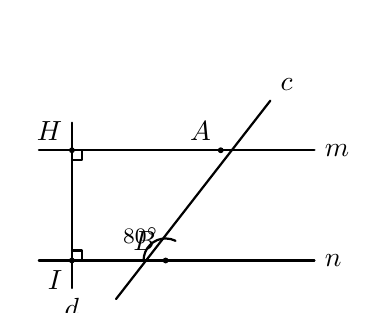
\begin{tikzpicture}[scale=0.7, line cap=round, line join=round]
    % Lines m and n
    \draw[thick] (-2.2, 2.0) -- (2.8, 2.0) node[right] {$m$};
    \draw[thick] (-2.2, 0) -- (2.8, 0) node[right] {$n$};
    % Line d perpendicular at H and I
    \draw[thick] (-1.6, 2.5) -- (-1.6, -0.5) node[below] {$d$};
    \filldraw[black] (-1.6, 2.0) circle (1.2pt) node[above left] {$H$};
    \filldraw[black] (-1.6, 0) circle (1.2pt) node[below left] {$I$};
    \draw[thick] (-1.6, 2.0) ++(0,-0.18) -- ++(0.18,0) -- ++(0,0.18);
    \draw[thick] (-1.6, 0) ++(0,0.18) -- ++(0.18,0) -- ++(0,-0.18);
    % Line c slanted cutting m at A, n at B
    \draw[thick] (2.0, 2.9) node[above right] {$c$} -- (-0.8, -0.7);
    \filldraw[black] (1.1, 2.0) circle (1.2pt) node[above left] {$A$};
    \filldraw[black] (0.1, 0) circle (1.2pt) node[above left] {$B$};
    % Angle ABI = 80
    \draw[thick] (0.1, 0) ++(180:0.4) arc (180:63.4:0.4);
    \node[font=\footnotesize] at (-0.35, 0.45) {$80^\circ$};
\end{tikzpicture}
}
\loigiai{
\textbf{a)} Ta có $m \perp d$ tại $H$ và $n \perp d$ tại $I$, do đó $m \parallel n$ (hai đường thẳng cùng vuông góc với một đường thẳng thứ ba thì song song với nhau).

\textbf{b)} Vì $m \parallel n$ nên $\widehat{cAH}$ và $\widehat{ABI}$ là hai góc đồng vị, suy ra $\widehat{cAH} = \widehat{ABI} = 80^\circ$.\par Mặt khác, $\widehat{mAc}$ và $\widehat{cAH}$ là hai góc kề bù nên: $\widehat{mAc} + \widehat{cAH} = 180^\circ \implies \widehat{mAc} = 180^\circ - 80^\circ = 100^\circ$.

\textbf{c)} Vì $AE$ là tia phân giác của $\widehat{cAH}$ nên $\widehat{cAE} = \dfrac{\widehat{cAH}}{2} = \dfrac{80^\circ}{2} = 40^\circ$.\par Vì $BF$ là tia phân giác của $\widehat{ABI}$ nên $\widehat{ABF} = \dfrac{\widehat{ABI}}{2} = \dfrac{80^\circ}{2} = 40^\circ$.\par Suy ra $\widehat{cAE} = \widehat{ABF} = 40^\circ$. Mà hai góc này ở vị trí đồng vị, do đó $AE \parallel BF$.
}
\end{ex}
\vspace{2mm}

\begin{ex}
Một cửa hàng nhập về $100$ xe hơi đồ chơi với giá gốc mỗi cái $300\,000$ đồng. Cửa hàng đã bán $65$ xe với giá mỗi cái lãi $30\%$ so với giá gốc; $35$ cái xe còn lại bán lỗ $7\%$ so với giá gốc. Hỏi sau khi bán hết $100$ xe hơi đồ chơi cửa hàng đó lãi hay lỗ bao nhiêu tiền?
\loigiai{
Tổng số vốn nhập $100$ chiếc xe là:\par \centerline{$100 \cdot 300\,000 = 30\,000\,000\text{ (đồng).}$}\par Số tiền thu được khi bán $65$ xe lãi $30\%$ là:\par \centerline{$65 \cdot 300\,000 \cdot (100\% + 30\%) = 65 \cdot 390\,000 = 25\,350\,000\text{ (đồng).}$}\par Số tiền thu được khi bán $35$ xe lỗ $7\%$ là:\par \centerline{$35 \cdot 300\,000 \cdot (100\% - 7\%) = 35 \cdot 279\,000 = 9\,765\,000\text{ (đồng).}$}\par Tổng số tiền thu về sau khi bán hết $100$ xe là:\par \centerline{$25\,350\,000 + 9\,765\,000 = 35\,115\,000\text{ (đồng).}$}\par Vì $35\,115\,000 > 30\,000\,000$ nên cửa hàng kinh doanh có lãi. Số tiền lãi là:\par \centerline{$35\,115\,000 - 30\,000\,000 = 5\,115\,000\text{ (đồng).}$}\par Vậy cửa hàng lãi $5\,115\,000$ đồng.
}
\end{ex}
\vspace{2mm}


\begin{center}
\rule{4cm}{0.4pt}\\
\textit{--- HẾT ---}
\end{center}
\end{document}
